% !TEX root = main.tex

\section{Implementierung}
%TODO Text ergänzen
\subsection{Sequentiell}
Die erste und einfachste Umsetzung des Entwurfs des Simulationsschritts wäre folgendes:
\begin{lstlisting}[language=C]
for (int i = 1; i < arrLen-1; i++)
	newval[i] = (2 * values[i]) - oldval[i] + c * (values[i-1] - (2 * values[i]) + values[i+1]);

for (int i = 1; i < arrLen-1; i++) 
{
	oldval[i] = values[i];
	values[i] = newval[i];
}
\end{lstlisting}

Dabei führen wir die Berechnung durch und kopieren anschließend die Werte jeweils einen "Schritt in die Vergangenheit". Das Kopieren der Arrays stellt unnötige Schreiboperationen dar. Eine Alternative hierzu ist der Toggle:

\begin{lstlisting}[language=C]
for (int i = 1; i < arrLen-1; i++)
{
	if (0 == mode)
		newval[i] = (2 * values[i]) - oldval[i] + c * (values[i-1] - (2 * values[i]) + values[i+1]);
	else if (1 == mode)
		oldval[i] = (2 * newval[i]) - values[i] + c * (newval[i-1] - (2 * newval[i]) + newval[i+1]);
	else
		values[i] = (2 * oldval[i]) - newval[i] + c * (oldval[i-1] - (2 * oldval[i]) + oldval[i+1]);
}
mode++;
if (2 < mode)
	mode = 0;
\end{lstlisting}

Hierbei wird kein Array auf ein anderes kopiert. Stattdessen wird die Bedeutung der Arrays verschoben. Initial werden auf newval die berechneten Werte geschrieben, values hält die gegenwärtigen Werte und oldval die ältesten Werte. Nach jedem Simulationsschritt wird dann die Bedeutung verschoben. Somit werden dann im nächsten Schritt die neuen Werte in oldval geschrieben, newval hält die gegenwärtigen Werte und values die ältesten Werte.\\
In Abbildung \ref{fig:toggle_swap} ist das Prinzip der Semantikverschiebung beim Toggle dargestellt.\\

\begin{figure}[H]
	\centering
	\smartdiagram[circular diagram:clockwise]{newval, values, oldval}
	\caption{Verschiebung der Semantik der Arrays}
	\label{fig:toggle_swap}
\end{figure}

\subsection{OpenMP}
Die Parallelisierung mit OpenMP ist nun sehr einfach. Dem Quellcode muss nur eine Zeile hingefügt werden und die Schleife wird dann parallelisiert:

\begin{lstlisting}[language=C]
#pragma omp parallel for
for (int i = 1; i < arrLen-1; i++)
[...]
\end{lstlisting}

In diesem Fall werden alle Variablen bis auf "i", da diese erst im Scope der Schleife deklariert wird, als global oder shared angesehen. Wir hatten hier die Vermutung, dass wir deshalb auch vom False-Sharing-Problem betroffen sein könnten. Aufgrund der Größe der Arrays und der Art wie OpenMP die Arrays aufteilt sollte dies aber nicht der Fall sein.

\subsection{OpenMPI}
%TODO


\subsection{Benutzeroberfläche}

\begin{figure}[H]
	\centering
	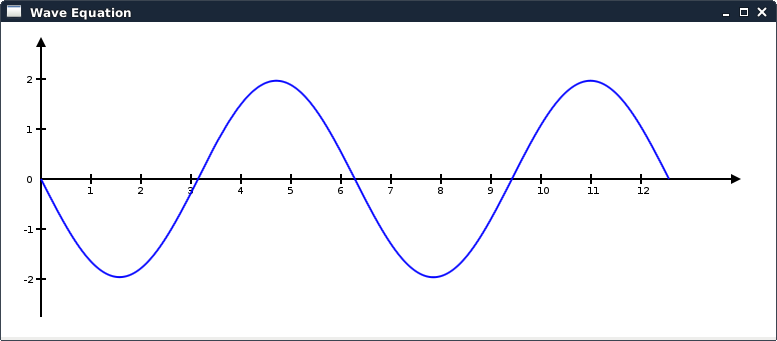
\includegraphics[width=0.9\textwidth]{pictures/gui}
	\caption{Graphical User Interface (GUI)}
	\label{fig:gui}
\end{figure}